\section{Laufzeitanalyse von Parsivald-Simulationen}
\label{runtime}

Für Parsivald-Simulationen ergeben sich verschiedene Einschränkungen, etwa in der Größe des Simulationsraumes oder der Laufzeit von MD-Simulationen, welche die Zahl der Parallelen Worker beschränken und die parallele Laufzeit erhöhen.
Nachfolgend wird deshalb eine Laufzeitanalyse von Parsivald unter Berücksichtigung diverser Größen durchgeführt.

Wie bei Laufzeitanalysen üblich, werden Laufzeiten mit $T$ bezeichnet und sollten nicht mit Temperaturen verwechselt werden.
Weiterhin bezeichnet die \textit{Größe} des Simulationsraumes oder der MD-Box nachfolgend die Fläche des Raumes anstatt des Volumens, da die Laufzeit im Parsivald-Modell unabhängig von der Höhe der Schicht ist.

\subsection{Ereignis-Laufzeit \texorpdfstring{$T_\text{E}$}{TE}}

Die Auswahl eines Ereignisses in KMC-Algorithmen ist mit einer Laufzeit~$T_\text{E}$ verbunden, die sich aus der Laufzeit von Suchoperationen $T_\text{KMC}$, der Laufzeit von Serialisierungen und Deserialisierungen zur Datenübertragung zwischen Host und Worker $T_\text{Ser.}$ und $T_\text{Des.}$ sowie der Laufzeit für die Konnektivitätsprüfung $T_\text{Konn.}$ zusammen setzt.
Damit bezeichnet sie die Zeit, die der Host-Prozess in parallelen Parsivald-Simulationen für ein Ereignis aufbringt.
\begin{equation}
T_\text{E} = T_\text{KMC} + T_\text{Ser.} + T_\text{Des.} + T_\text{Konn.}
\end{equation}
Aufgrund des Buffer-Verhaltens der C-Bibliothek sind $T_\text{Ser.}$ und $T_\text{Des.}$ bereits minimal, sodass Ansatzpunkte für Optimierungen nur bei den KMC-Suchoperationen (Abschnitt~\ref{datastructures}) sowie bei der Konnektivitätsprüfung, welche mit \BigO{N^2} zur Zahl der Atome in der MD-Box $N$ am stärksten skaliert, bestehen.

\subsection{Ereignis-Durchsatz \texorpdfstring{$R_\text{E}$}{RE}}

Als Ereignis-Durchsatz $R_\text{E}$ wird nachfolgend die Zahl der vom Host zur MD-Berechnung maximal bereit gestellten Ereignisse pro Zeiteinheit bezeichnet.
Damit handelt es sich eigentlich um eine Rate von Ereignissen, die jedoch nicht mit der Ereignisrate aus dem KMC-Formalismus (Abschnitt~\ref{kmc}) verwechselt werden sollte.
In der aktuellen Implementierung führt ein einziger serieller Host-Prozess alle Vor- und Nachbereitungen von Ereignissen durch, weshalb gilt:

\begin{equation}
  R_\text{E} = \frac{1}{T_\text{E}}
\end{equation}

\subsection{MD-Laufzeit \texorpdfstring{$T_\text{MD}$}{TMD}}

Die Zeit, die ein Worker zur MD-Simulation eines Ereignisses aufbringt, wird im Folgenden als MD-Laufzeit $T_\text{MD}$ bezeichnet.
Sie ist hauptsächlich von den benutzten Kraftfeldern abhängig, wird jedoch auch durch die durchgeführten MD-Operationen, die Relaxationszeit, sowie die Größe der MD-Box und die damit verbundene Zahl der Atome beeinflusst.
Vom KMC-Algorithmus ist sie hingegen unabhängig.

\subsection{Worker-Laufzeit \texorpdfstring{$T_\text{worker}$}{Tworker}}

Die Worker-Laufzeit ergibt sich aus der MD-Laufzeit und der Zeit zur Deserialisierung der Anfangsbedingungen und zur Serialisierung der Ergebnisse.
Da hier die MD-Laufzeit dominiert, wird diese zur Berechnung abgeleiteter Größen genutzt.
\begin{equation}
  T_\text{worker} = T_\text{Ser.} + T_\text{Des.} + T_\text{MD} \approx T_\text{MD}
\end{equation}

\subsection{Serielle Laufzeit \texorpdfstring{$T_1$}{T1}}

Die serielle Laufzeit $T_1$ bezeichnet die Laufzeit eines Programmes unter Nutzung eines einzigen Prozesses.
Damit ist sie von der vernachlässigbaren Laufzeit zur einmaligen Vorbereitung $T_\text{start}$ und den Ereignis- und MD-Laufzeiten $T_\text{E}$ und $T_\text{MD}$ sowie der Zahl der Ereignisse $N_\text{E}$ abhängig.

\begin{align}
  T_1 & = T_\text{start} + N_\text{E} \cdot (T_\text{E} + T_\text{MD}) \\
      & \approx N_\text{E} T_\text{E} + N_\text{E} T_\text{MD}
\end{align}

\subsection{Anzahl der parallelen Prozesse \texorpdfstring{$p$}{p}}

Parsivald-Simulationen werden in einen Host-Prozess und $p-1$ Workerprozesse eingeteilt, woraus sich insgesamt $p$ parallele Prozesse ergeben.
Die oberen Schranken $p_\text{max}$ liegen dabei in Abhängigkeit der Größe des Simulationsraumes in der maximalen Abdeckung der Oberfläche mit MD-Boxen sowie im Ereignis-Durchsatz des Host-Prozesses.
Für kleine Simulationsräume lässt sich die maximale Anzahl von Ereignissen $p_\text{max,1}-1$ aus der dichtesten Packung von nicht-überlappenden, meist quadratischen MD-Boxen der Breite $w_\text{MD}$, Tiefe $d_\text{MD}$ und Fläche $A_\text{MD} = w_\text{MD} \cdot d_\text{MD}$ im Simulationsraum ($w_\text{sim}$, $d_\text{sim}$, $A_\text{sim}$) abschätzen:
\begin{equation}
  p_\text{max,1} = \left\lfloor\frac{w_\text{sim}}{w_\text{MD}}\right\rfloor \cdot \left\lfloor\frac{d_\text{sim}}{d_\text{MD}}\right\rfloor + 1 \approx \left\lfloor\frac{A_\text{sim}}{A_\text{MD}}\right\rfloor + 1
  \label{eq:pmax1}
\end{equation}
Bei großen Simulationsräumen ergibt sich die obere Schranke aus dem Ereignis-Durchsatz des Hauptprozesses in Verbindung mit der Laufzeit der MD-Simulationen:
\begin{equation}
  p_\text{max,2} = R_\text{E} \cdot T_\text{MD} + 1 = \frac{T_\text{MD}}{T_\text{E}} + 1
  \label{eq:pmax2}
\end{equation}
Somit bestimmt sich $p_\text{max}$ als Minimum der beiden oberen Schranken $p_\text{max,1/2}$ .
\begin{align}
  %% p_\text{max} & = \min(p_\text{max,1}, p_\text{max,2}) \\
  %%              & = \min\left(\left\lfloor\frac{A_\text{sim}}{A_\text{MD}}\right\rfloor, \frac{T_\text{MD}}{T_\text{E}}\right)
  p_\text{max} = \min\left(\left\lfloor\frac{A_\text{sim}}{A_\text{MD}}\right\rfloor, \frac{T_\text{MD}}{T_\text{E}}\right) + 1
  \label{eq:pmax}
\end{align}

\subsection{Workerdichte \texorpdfstring{$\rho_\text{worker}$}{rhoworker}}

Ein Parsivald-spezifisches Leistungsmaß ergibt sich mit der Workerdichte, welche das Verhältnis der mittleren Anzahl der aktiven Worker $p-1$ zur maximalen Zahl gleichzeitiger Ereignisse im Simulationsraum $p_\text{max,1}-1$ beschreibt und somit auch für verschiedene Kraftfelder und Substratgrößen vergleichbar ist.
Aufgrund der stochastischen Verteilung der Ereignisorte werden in Simulationsläufen nur zwischen \SI{10}{\percent} und \SI{40}{\percent} für $\rho_\text{worker}$ erreicht (siehe Anhang~\ref{appendix_rsamaxdensity}).
\begin{equation}
  \rho_\text{worker} = \frac{p - 1}{p_\text{max,1} - 1}
  \label{eq:workerdensity}
\end{equation}

\subsection{Parallele Laufzeit \texorpdfstring{$T_p$}{Tp}}

Die parallele Laufzeit $T_p$ bezeichnet die Laufzeit eines Programmes unter Nutzung von $p$ parallelen Prozessen.
Neben den MD-Workern muss dabei auch der Hauptprozess beachtet werden, der die KMC-Operationen verwaltet, sodass die MD-Simulationen auf nur $p-1$ Prozesse aufgeteilt werden.
Durch Synchronisation von Hauptprozess und Workerpools bildet sich die parallele Laufzeit aus dem Maximum der Host- und Worker-Laufzeiten.

\begin{equation}
  T_p = T_\text{start} + \max\left(N_\text{E} T_\text{E}, \frac{N_\text{E} T_\text{MD}}{p-1}\right) \approx \frac{N_\text{E} T_\text{MD}}{p-1}
  \label{eq:runtime}
\end{equation}

\subsection{Speedup \texorpdfstring{$S_p$}{Sp}}

Beim Speedup handelt es sich um ein für Laufzeitanalysen übliches Maß, welches sich aus dem Verhältnis der linearen Laufzeit zur parallelen Laufzeit bildet.
\begin{align}
  S_p & = \frac{T_1}{T_p} = \left(p-1\right) \frac{\left(T_\text{E} + T_\text{MD}\right)}{T_\text{MD}} \\
      & = p - \frac{p_\text{max,2} - p}{p_\text{max,2} - 1}
\end{align}
Bei Parsivald-Läufen mit wenigen Workern ist der Speedup somit sublinear, nimmt aber für große Simulationsräume mit $p = p_\text{max,2}$ theoretisch einen idealen Speedup von $S_\text{max} = p_\text{max,2} = p$ an.
%% Dabei ist nicht $S_\text{max}$ selbst maximal, sondern die Zahl der parallelen Prozesse.

\subsection{Parallele Effizienz \texorpdfstring{$E_p$}{Ep}}

Die parallele Effizienz $E_p$ ist als Verhältnis aus dem Speedup $S_p$ zur Zahl der Prozesse $p$ definiert:
\begin{equation}
  E_p = \frac{S_p}{p} = 1 - \frac{p_\text{max,2} - p}{p (p_\text{max,2} - 1)}
\end{equation}
Somit ergibt sich für $p = p_\text{max,2}$ mit $E_\text{max} = 1$ eine ideale Effizienz, die auf volle Auslastung für $p_\text{max}$ Prozesse bei vernachlässigbarem Overhead hinweist.

%% \subsection{Abschätzung des parallelen Anteils \texorpdfstring{$P$}{P} (Parallelisierbarkeit)}

%% Aus den oben gegebenen Formeln lässt sich der serielle Anteil $S$ der Laufzeit anhand der maximalen Zahl der Worker $p = p_\text{max,2}$ abschätzen:
%% \begin{equation}
%%   S = \frac{T_\text{E}}{T_\text{MD} + T_\text{E}} = \frac{1}{p + 1}
%% \end{equation}
%% Aus der Beziehung $S + P = 1$ ergibt sich eine Parallelisierbarkeit $P$ von Parsivald aus der Zahl der Worker $p$ wie folgt:
%% \begin{equation}
%%   P = \frac{p}{p+1}
%% \end{equation}

\subsection{Auswertung der Laufzeitparameter}
\label{runtimeanalysis}

Die Parallelisierung von Parsivald-Simulationen lässt sich über die Größe der als quadratisch angenommen Simulationsräume $w_\text{sim}$, die Ereignis-Laufzeit $T_\text{E}$ und die MD-Laufzeit $T_\text{MD}$ beeinflussen.
Einen geringeren Einfluss haben die Größe der MD-Box $w_\text{MD}$ und die mittlere Workerdichte~$\rho_\text{worker}$ des Prozesses, welche ergänzend in Anhang~\ref{appendix_runtime} untersucht werden.
Im allgemeinen Fall muss ein Gleichgewicht zwischen $T_\text{E}$, $T_\text{MD}$, $w_\text{sim}$ und $p$ gefunden werden.

Das Skalierungsverhalten von Parsivald teilt sich anhand der Raumgröße $w_\text{sim}$ in zwei Bereiche ein.
Für \textit{kleine Räume} mit $w_\text{sim} \le w_\text{eff}$ determiniert $p_\text{max,1}$ das Skalierungsverhalten, wohingegen für \textit{große Räume} ($w_\text{sim} \ge w_\text{eff}$) $p_\text{max,2}$ dominiert.
Die effiziente Raumgröße $\le w_\text{eff}$ entspricht dabei einer kritischen Raumgröße, an der ein Knick in den Abbildungen~\ref{fig:densitymaxsize},\ref{fig:workersbytime} und~\ref{fig:runtimebytime} erkennbar ist.

Die effiziente Größe $w_\text{eff}$ lässt sich anhand der maximalen Workerdichte $\rho_\text{worker,max}$ bestimmen.
Liegt diese oberhalb einer aus Erfahrungen gewonnenen Grenze von \SI{10}{\percent}, wird von einem effizienten Prozess im Sinne der parallelen Effizienz ausgegangen.
Es gilt dann aufgrund der Beziehungen aus Gleichungen~\ref{eq:pmax} und~\ref{eq:workerdensity}:%legitequationreference
\begin{align}
  w_\text{eff} & \sim T_\text{MD}     \\
  w_\text{eff} & \sim T_\text{E}^{-1}
\end{align}
Für die aktuelle Implementierung ergibt sich für EAM-Potentiale mit \SI{5}{\second} MD-Laufzeit die effiziente Größe als $w_\text{eff} = \SI{150}{\nano\meter}$ und für ReaxFF-Potentiale mit $T_\text{MD}=\SI{50}{\second}$ als $w_\text{eff} = \SI{400}{\nano\meter}$.
Unter Optimierung des Hostprozesses zu $T_\text{E} = \SI{3}{\milli\second}$ sind theoretisch \SI{2x2}{\micro\meter} große Räume effizient berechenbar, doch ist hierbei die Zahl der notwendigen Prozessoren zu beachten.

\begin{figure}[p]
  \captionsetup[subfigure]{singlelinecheck=false}
  \def\subfigwidth{7cm}
  \begin{subfigure}[t]{\subfigwidth}
    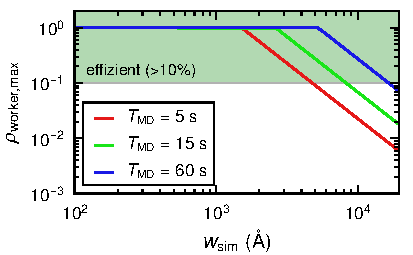
\includegraphics[width=\textwidth]{densitybymdtime}
  \end{subfigure}
  \hfill
  \begin{subfigure}[t]{\subfigwidth}
    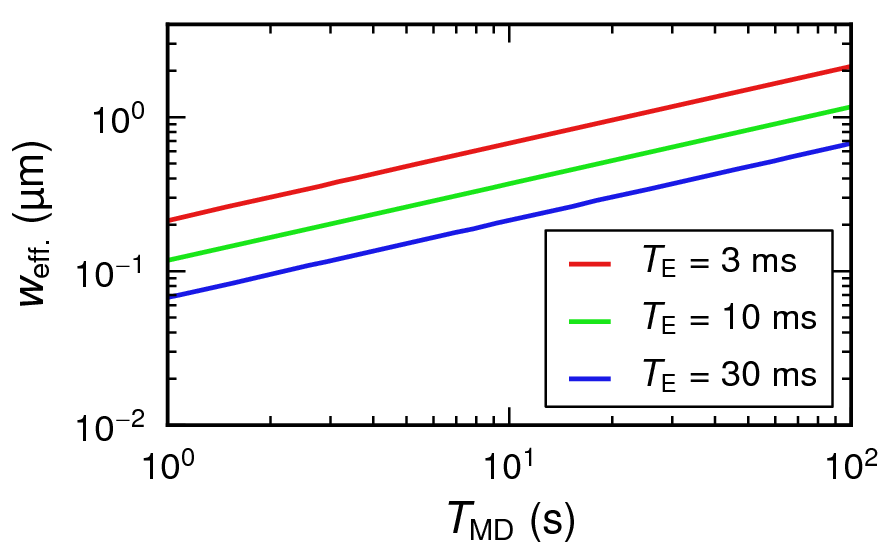
\includegraphics[width=\textwidth]{maxsizebymdtime}
  \end{subfigure}

  \caption[$\rho_\text{worker}$ und $w_\text{eff}$ in Abhängigkeit von $T_\text{MD}$]{Einfluss der MD-Laufzeit auf die maximale Workerdichte und das Maximum der Simulationsgröße für effiziente Rechnungen ($\rho_\text{worker} > \SI{10}{\percent}$)}
  \label{fig:densitymaxsize}

\end{figure}

Dieser Einfluss ist auch in Abbildung~\ref{fig:workersbytime} zu erkennen, bei der eine Verschiebung von $w_\text{eff}$ mit einer Verschiebung des Knicks einher geht und somit mehr Prozesse für große Räume zulässt.
Durch Extrapolierung sind Werte von mehr als \num{10000} Prozessen zur effizienten Simulation von \SI{1x1}{\micro\meter} großen Räumen ersichtlich, welche die technischen Grenzen aktueller Rechencluster übersteigen.
Die maximale Zahl der Prozesse in kleinen Räumen wird hingegen ausschließlich über die Größe der MD-Box $w_\text{MD}$ bestimmt, welche zur Reduktion der Gesamt-Laufzeit nach Möglichkeit minimal gewählt wird.

\begin{figure}[p]

  \captionsetup[subfigure]{singlelinecheck=false}
  \def\subfigwidth{7cm}
  \begin{subfigure}[t]{\subfigwidth}
    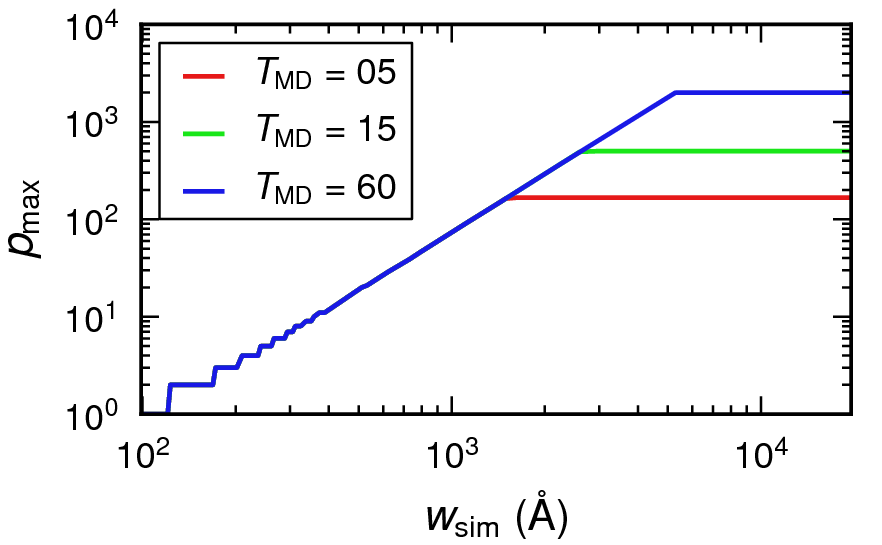
\includegraphics[width=\textwidth]{workersbymdtime}
  \end{subfigure}
  \hfill
  \begin{subfigure}[t]{\subfigwidth}
    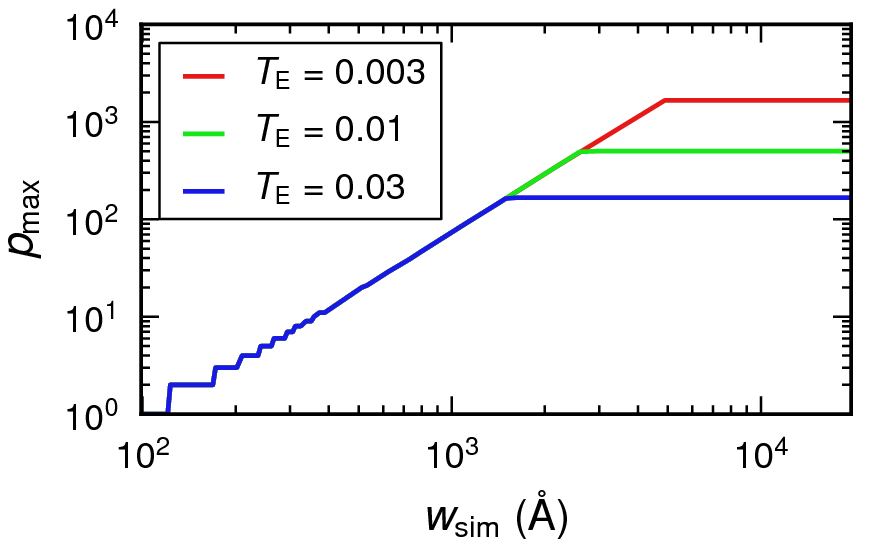
\includegraphics[width=\textwidth]{workersbykmctime}
  \end{subfigure}

  \caption[$p_\text{max}$ in Abhängigkeit von $T_\text{E}$ und $T_\text{MD}$]{Einfluss der Ereignis-Laufzeit $T_\text{E}$ und der MD-Laufzeit $T_\text{MD}$ auf die maximale Zahl paralleler Prozesse $p_\text{max}$}
  \label{fig:workersbytime}

\end{figure}

Für die Gesamt-Laufzeit ergibt sich ein konstantes Skalierungsverhalten für kleine Räume, während große Räume lineares Verhalten mit der Größe der Oberfläche zeigen.
Die Laufzeit $T_p$ ist also unabhängig von $w_\text{sim}$, solange $w \le w_\text{eff}$ gilt.
Für große Räume mit $w_\text{sim} > w_\text{eff}$ ist die Gesamt-Laufzeit $T_p$ außerdem von der MD-Laufzeit unabhängig, was sich durch die gegenseitige Aufhebung von $T_p \sim T_\text{MD}$ und $p_\text{max} \sim T_\text{MD}$ über die Beziehung $T_p \sim p^{-1}$ ergibt.
Mit der MD-Zeit steigt also die maximale Zahl der Worker linear, wodurch mehr Ereignisse gleichzeitig bearbeitet werden und so alle zu simulierenden Ereignisse des Parsivald-Zyklus' theoretisch in der selben Zeit $T_p$ abgearbeitet werden können, sofern eine ausreichende Zahl von Prozessen zur Verfügung steht.

\begin{figure}[p]

  \captionsetup[subfigure]{singlelinecheck=false}
  \def\subfigwidth{7cm}
  \begin{subfigure}[t]{\subfigwidth}
    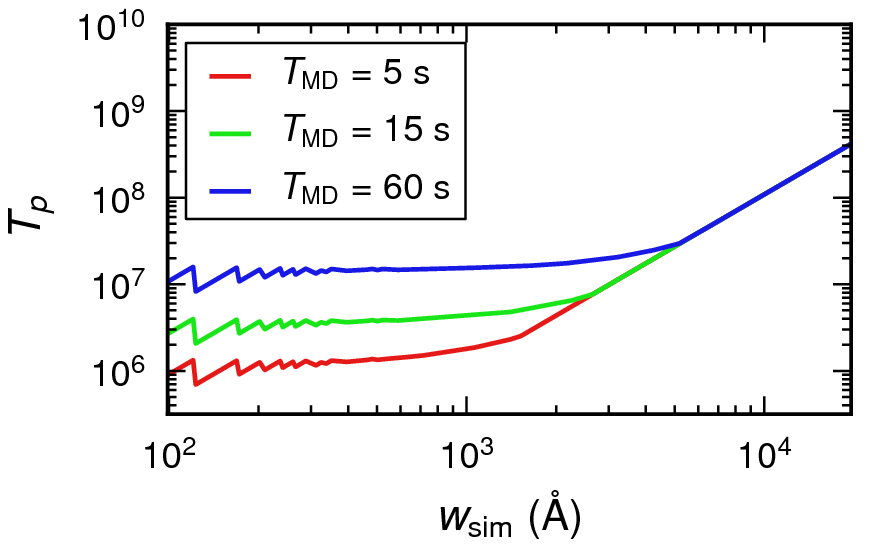
\includegraphics[width=\textwidth]{runtimebymdtime}
  \end{subfigure}
  \hfill
  \begin{subfigure}[t]{\subfigwidth}
    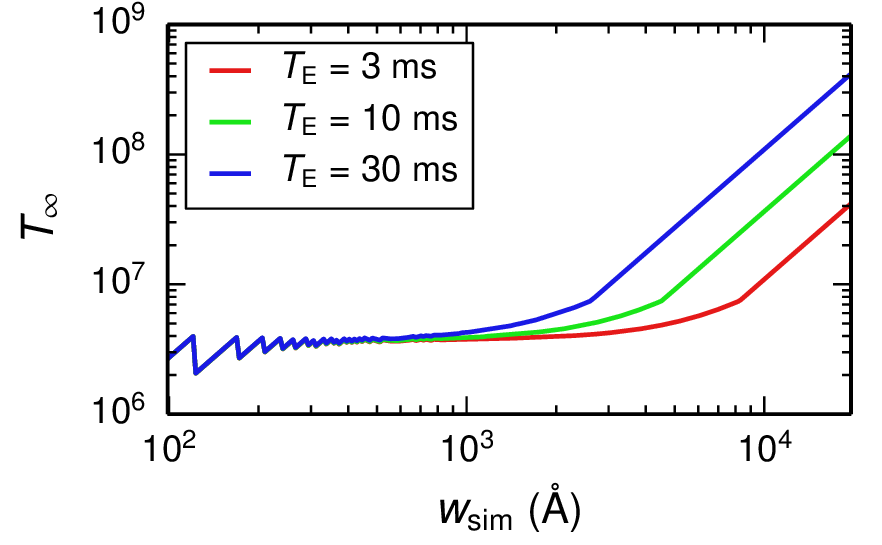
\includegraphics[width=\textwidth]{runtimebykmctime}
  \end{subfigure}

  \caption[$T_\infty$ in Abhängigkeit von $T_\text{E}$ und $T_\text{MD}$]{Einfluss der Ereignis-Laufzeit $T_\text{E}$ und der MD-Laufzeit $T_\text{MD}$ auf die minimale Laufzeit $T_\infty$ einer Parsivald-Simulation}
  \label{fig:runtimebytime}

\end{figure}

\subsection{Fazit}

Eine theoretische Analyse Laufzeit und Skalierbarkeit von Parsivald zeigt, dass für kleine Simulationsräume konstante parallele Laufzeiten $T_p$ unabhängig von der Größe der Oberfläche ermöglicht werden, wohingegen für große Simulationsräume eine ideale parallele Effizienz $E_\text{max} = 1$ für bis zu $p_\text{max}$ parallele Prozesse möglich ist.
Die Grenze zwischen diesen Bereichen lässt sich als effiziente Raumgröße $w_\text{eff}$ ermitteln, welche den größten Simulationsraum beschreibt, der in minimaler Laufzeit simuliert werden kann.
Damit eignet sich Parsivald für effiziente atomistische Simulationen von Abscheidungsprozessen.

